\section{Model 2: Computer Model}

In this Model,we will establish a three-dimensional Model
based on the model 1.

\begin{figure}[!htb]
\centering
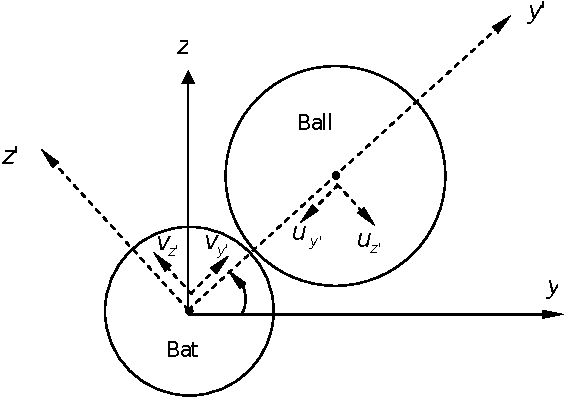
\includegraphics[width=0.6\textwidth]{computer.pdf}
\caption{\label{computermodel}Initial vertical configuration of the bat/ball collision. (Where $x$ and $x'$ axis perpendicular to the paper outwards, the figure is not drawn)}
\end{figure}


As the Figure \ref{computermodel} shows, the momentum of the $y'$  direction between the bat and ball before and after the collision is conserved:

\[
Mv'_{y0}+mu'_{y0}=Mv'_y+mu'_y
\]
On the assumption that the rotational kinetic energy of the ball is negligible when compared to the translational kinetic energy. Conserving angular momentum between the bat and the ball during the collision produces

\[
I_0(\omega-\omega')+Bm(u'_y-u_y)=0
\]

The COR is defined as

\[
e=\frac{u'_y-v'_y}{u'_{y0}-v'_{y0}}
\]

In fact��the above model concerning the velocity fluctuation of the  $y'$ direction is the previous simple model which is already established. But in the computer model, we do not take into consideration the friction effect of the instant of collision, so we have the following equations which are

\[
v'_z=v'_{z0}, u'_z=u'_{z0}
\]

\[
v'_x=v'_{x0}=0, u'_x=u'_{x0}
\]

In fact, the friction effect will make the velocity change in both the $x'$  direction and the $z'$ direction, and could also cause the rotational motion of the ball happens. However, we believe that ignoring the role of friction will not make our results have larger errors. And by doing this, we gain the result that the sweet spot is not at the end of the bat once again, it proves our model is correct and feasible.

We proceed from the simple model to establish a general three-dimensional model, and use the computer to go on with analog simulation. In each analog simulation of our model, we will make the following parameters be set to normally distributed random numbers, thus we can simulate the process of the batting, and this will be closer to the reality. Simultaneously, we can also use the process of the batting to respond the different levels about the players by the setting a random numbers, especially the typical value and the variance. As a result, when we set the random numbers preferable can it respond to people with a higher level of batting, conversely, it will reflects the player to be a beginner. The parameters as shown followed:

\begin{itemize}
\item The ball's initial velocity (including direction).

\item The bat's initial velocity (including direction).

\item The distance between the point of impact and the sweet spot determined by model 1.

\item The height from hitting position to the ground.

\item The $\theta$ angle in the figure \ref{computermodel}.
\end{itemize}

\subsection{The effect of the sweet spot of the corked bat}

To analyze the effects of the different types of the bats which are unmodified or corked when hit the baseball, we created different simulations batting by varying our parameters. We then ran each simulations batting strategy on these different parameters to get the hitting ranges for each bat, and our initial inference is that the corked bat will be better than the unmodified bat for the latter can not make the player control easier when hitting the baseball. In particular, our goal through these simulations is to determine which of the bats has the greatest effect of the sweet spot on the simulated performance of the different structures. As a result, we get the figures to explain whether the unmodified bat or the corked bat is better to be used, as shown in the Figure \ref{Fieldcorked}.

\begin{figure}[!htb]
\centering
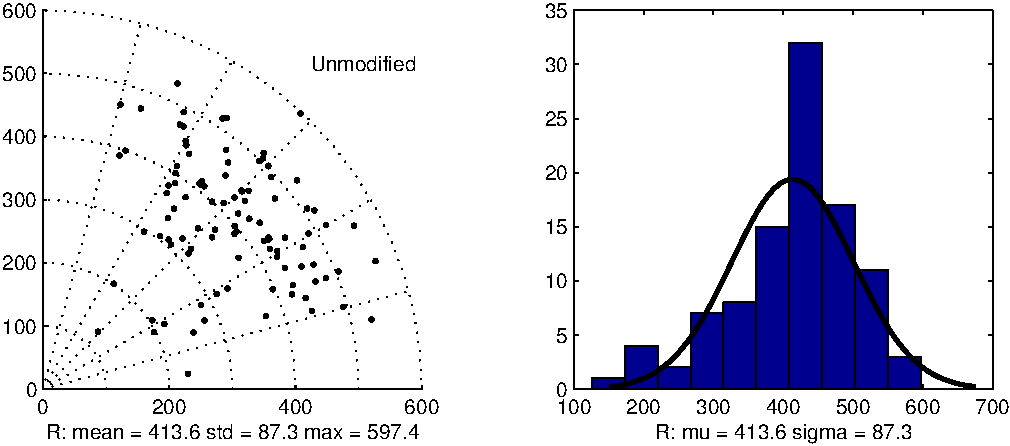
\includegraphics[width=0.71\textwidth]{unmodifiedm2.pdf}\\
.\\
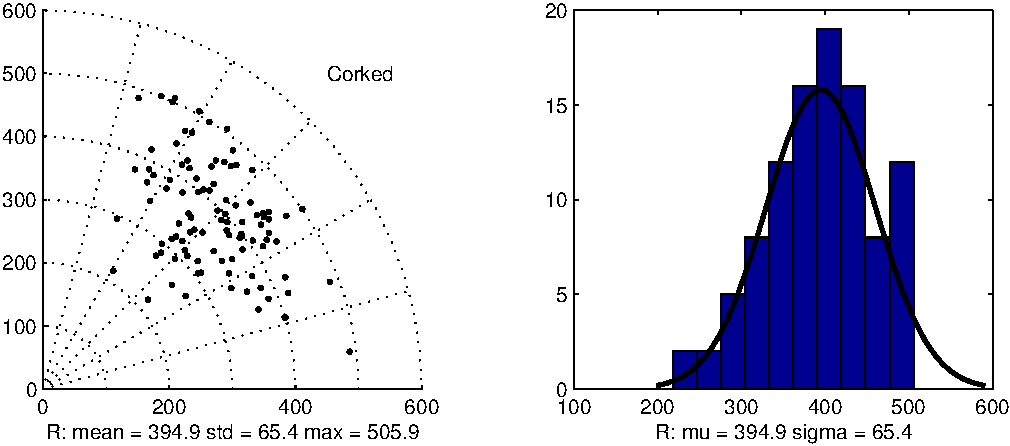
\includegraphics[width=0.71\textwidth]{corkedm2.pdf}\\
\caption{\label{Fieldcorked}Field locations of the corked bat bats baseballs and its range distribution. Both the above and the under figure on the left side represent respectively the field locations of batted baseballs, and both the above and the under figure on the right reflect respectively the distribution of the hitting range which is from (0,0) to the baseball's landing point.}
\end{figure}

Note: Because when using the corked bat to hit the baseball could make the player have a longer reaction time to control the motion of the baseball [see the above explanation in the Plane Mechanics Model] , the standard deviation about the ball hits the vicinage of the sweet spot (namely, the sweet spot zone) that we get by using the unmodified bat is larger than using the corked bat when we make simulation, that is to say that the probability of the baseball hits the sweet spot zone is much larger when using a corked bat. It confirms that ``corking" a bat could enhance the "sweet spot" effect. For this reason, the principle of the athletic and fair play can not be represented in the baseball game.

Although the speed of the baseball was shot out of reduces, on the other hand, as long as the second or the third rampart has enough time to be able to score, the corked bat is a better one. Therefore, a corked bat may be only used to make ball control to get scores better. However, the current problem is that no one knows whether it is real that a corked bat acts worse than the uncorked, so in lots of baseball games the corked bat are still not allowed to use. Maybe the corked bat is able to improve its breakage rate and reduce the difficulty of the game, so for the purpose of the principle of safe and fair play, the corked bat is prohibited.

\subsection{The differences between the wood and aluminum bats}

For good measure, with the view of explaining the different effects between the wood and metal bats, we have also taken into consideration some of the above parameters to talk about the differences between the wood and metal bats. Furthermore, by changing the different parameters, we produce the plots measuring the effectiveness of the various materials bat concerning the speed when the two types of the bats hit the baseball, field locations of the baseball's landing sites and the distributions of the baseball's hitting range and so on by conducting a computer simulation. In the following article, we will show the differences by means of the figure \ref{Fieldwood}.

\newpage

\begin{figure}[!htb]
\centering
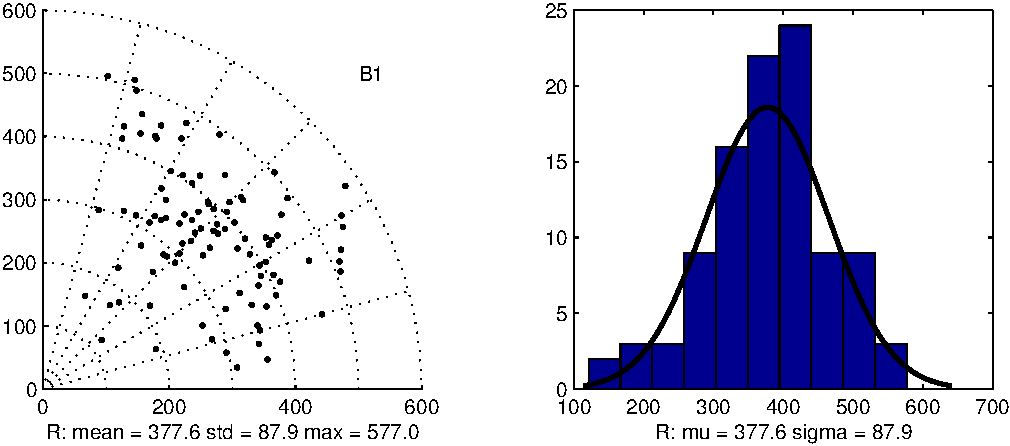
\includegraphics[width=0.71\textwidth]{b1.pdf}\\
.\\
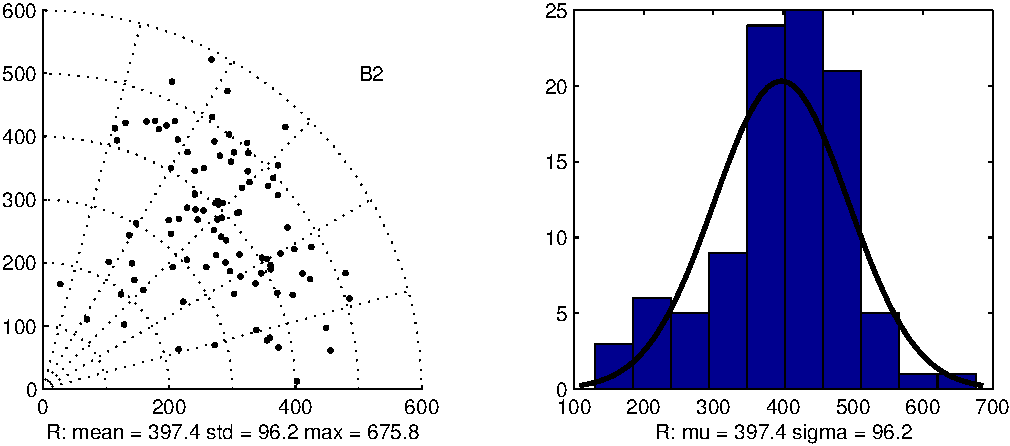
\includegraphics[width=0.71\textwidth]{b2.pdf}\\
.\\
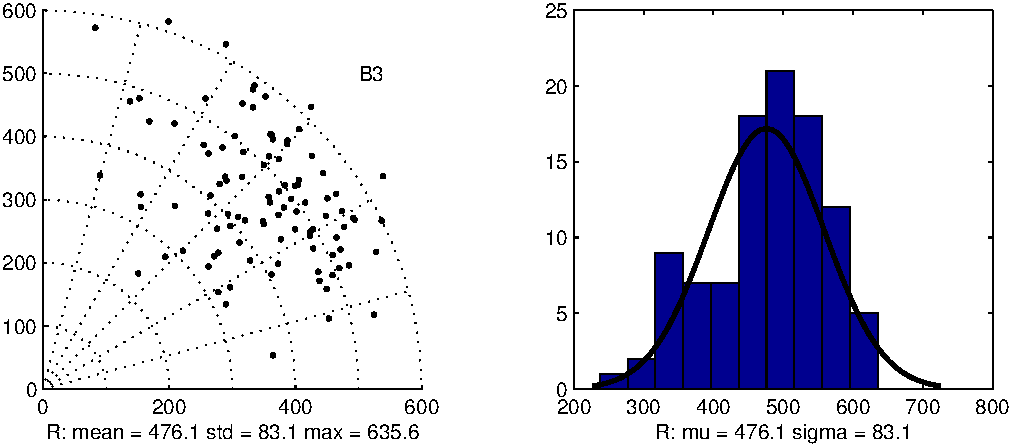
\includegraphics[width=0.71\textwidth]{b3.pdf}\\
.\\
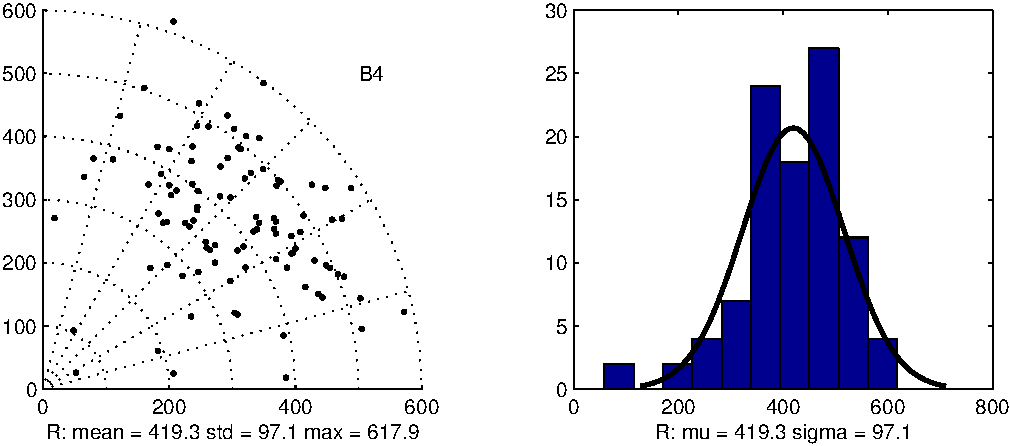
\includegraphics[width=0.71\textwidth]{b4.pdf}\\
\end{figure}

\begin{figure}[!htb]
\centering
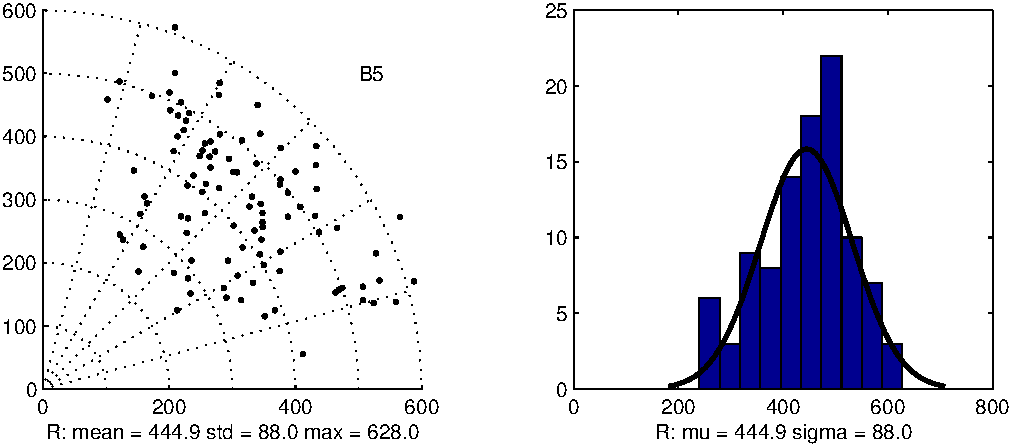
\includegraphics[width=0.71\textwidth]{b5.pdf}\\
.\\
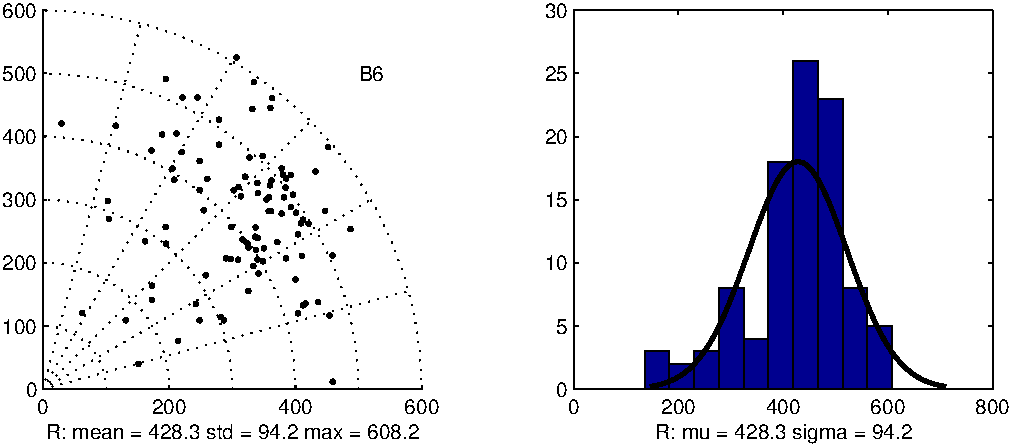
\includegraphics[width=0.71\textwidth]{b6.pdf}\\
.\\
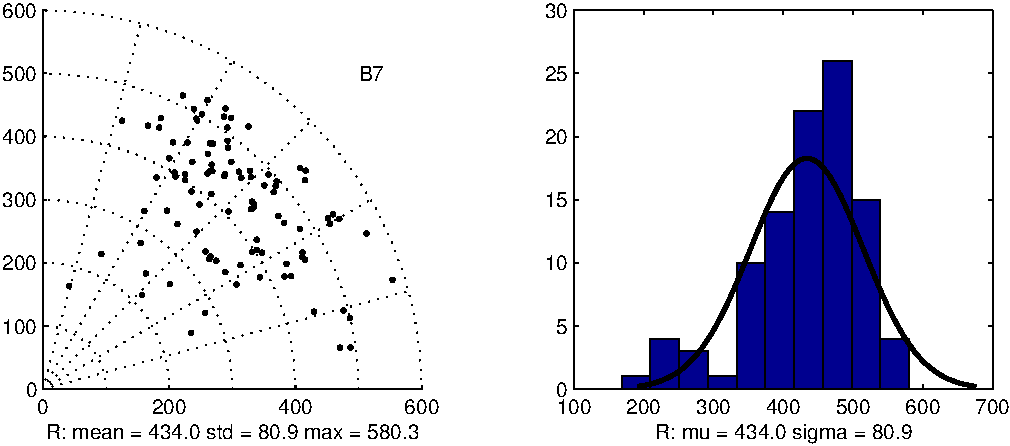
\includegraphics[width=0.71\textwidth]{b7.pdf}\\
\caption{\label{Fieldwood}Field locations of the wood(B1-B4) and metal(B5-B7) bats batted baseballs and their range distribution. Both the above and the under figure on the left side represent respectively the field locations of batted baseballs , and both the above and the under figure on the right reflect respectively the distribution of the hitting range which is from (0,0) to the baseball's landing point.}
\end{figure}

As everyone knows that in the same conditions, the aluminum bat hits the baseball with a longer distance than the wood bat does in general(bat B3 is performance different in evidence from the other wood bats, this responds our previous conclusion that its special structure makes it different, see model 1 and figure \ref{correspondingparameters}). From the figure we can see that the average velocity is 20 inches faster when hit by the aluminum than the wood bat, but the standard deviation between the two different kind of the bats is almost identical. However, in order to improve the competitive nature of the baseball games, in the rules of the baseball game the aluminum bat is prohibited to use.

